\chapter{Реализация}
\section{Численное интегрирование}
В работе рассматриваются два метода приближенного вычисления интегралов
(\ref{simpson}, \ref{gauss}).

Все приемы численного интегрирования [\ref{samarskiy}] основаны на  замене определенного интеграла 
\begin{equation}
	I = \int\limits_a^b f(x)\,dx
\end{equation}
конечной суммой
\begin{equation}
	I_n = \sum\limits_{k=0}^n c_k f(x_k),
\end{equation}

где $c_k$~--- числовые коэффициенты и $x_k$~---точки отрезка $[a,b]$, $k=0, 1, \ldots, n$.
При этом интеграл по переменному верхнему пределу берется так: Выбирается разбиение возможных значений верхнего предела
с определенным шагом. Внутри этого отрезка оба предела интеграла являются определенными и выбирается одна из ниже описанных формул.

\subsection{Метод Симпсона\label{simpson}}
При аппроксимации интеграла заменим подынтегральную функцию $f(x)$ параболой, проходящей через точки
($x_j, f(x_j) $), $j=i-1, i-0.5, i$. Подробный вывод формул представлен в [\ref{samarskiy}]. Приведем окончательную формулу:
\begin{equation}
\int\limits^b_a f(x)\,dx \approx \dfrac{b-a}{6N}\left[f_0 +f_{2N}+2(f_2+f_4+\ldots+f_{2N-2})+4(f_1+f_3+\ldots+f(2N-1))\right],
\end{equation}

где $2N$~--- количество узлов одномерной сетки c шагом $h$, $f_i$~--- значение функции $f$ в точке $x_i$. $x_i = a+kh$

\subsection{Метод Гаусса\label{gauss}}
Повысить точность вычисления численного интеграла можно не только с помощью уменьшения шага интегрирования, но и за счет 
выбора определенных точек интегрирования. Уменьшение шага ведет в пропорциональному увеличению времени работы программы, что не
приемлемо по времени работы при сильно увеличивающейся точности.

Метод Гаусса описывает способ нахождения специальных точек интегрирования, при этом в разложении интеграла используются квадратурные
формулы наивысшей алгебраической точности.
Изначально при методе Гаусса рассматривается канонический интеграл:
\begin{equation}
\int\limits_{-1}^1 f(x)\, dx = \sum\limits_{i=1}^n w_i f(x_i)
\end{equation}

Для перехода к произвольному интервалу можно воспользоваться следующей заменой:
\begin{equation}
\int_a^b f(x)\,dx = \frac{b-a}{2} \int_{-1}^1 f\left(\frac{b-a}{2}z 
+ \frac{a+b}{2}\right)\,dz \approx \frac{b-a}{2} \sum_{i=1}^n w_i f\left(\frac{b-a}{2}z_i + \frac{a+b}{2}\right).
\end{equation}

В работах [\ref{samarskiy}, \ref{gauss_book}, \ref{gauss_article}] подробно описан вывод и доказательство корректности формул, поэтому просто приведем таблицу 
ключевых значений для 1,2,3,4,5-ти точечного метода.

\begin{center}

\renewcommand{\arraystretch}{2}
\begin{tabular}{|c|c|c|}
\hline
Кол-во точек    & $x_i$ & $w_i$ \\
\hline\hline
1    & 0  & 2\\[5pt] \hline
2     & $\pm\frac{\sqrt{3}}{3}$   & 1 \\[5pt] \hline
\multirow{2}{*}{3}    & 0  & $\frac 89$\\[5pt] \cline{2-3}
& $\pm \sqrt{\frac 3 5}$  & $\frac 5 9$\\[5pt] \hline

\multirow{2}{*}{4}    & $\pm\sqrt{\Big( 3 - 2\sqrt{\frac65} \Big)/7}$ & $\frac{18+\sqrt{30}}{36}$\\[5pt] \cline{2-3}
& $\pm\sqrt{\Big( 3 + 2\sqrt{\frac{6}{5}} \Big)/7}$ & $\frac{18-\sqrt{30}}{36}$\\[5pt] \hline

\multirow{3}{*}{5}    & 0 & $\frac{128}{225}$\\[5pt] \cline{2-3}
& $\pm\frac13\sqrt{5-2\sqrt{\frac{10}{7}}}$ & $\frac{322+13\sqrt{70}}{900}$\\[5pt] \cline{2-3}
& $\pm\frac13\sqrt{5+2\sqrt{\frac{10}{7}}}$ & $\frac{322-13\sqrt{70}}{900}$\\[5pt] \hline

\end{tabular}
\label{gauss_table}
\end{center}

В работе использовался пятиточечный метод и окончательная формула принимает вид:
\begin{equation}
\begin{split}
	\int\limits_a^b f(x)\,dx =  128/255 f(\dfrac{a+b}{2})+
  \dfrac{322+13\sqrt{70}}{900}\cdot f\left(\dfrac{a+b}{2} + \dfrac 13\cdot \sqrt{5-2\sqrt{\dfrac{10}{7}}}\cdot\dfrac{b-a}{2}\right) +\\
  \dfrac{322+13\sqrt{70}}{900}\cdot f\left(\dfrac{a+b}{2} - \dfrac 13\cdot \sqrt{5-2\sqrt{\dfrac{10}{7}}}\cdot\dfrac{b-a}{2}\right) +\\
  \dfrac{322-13\sqrt{70}}{900}\cdot f\left(\dfrac{a+b}{2} + \dfrac 13\cdot \sqrt{5+2\sqrt{\dfrac{10}{7}}}\cdot\dfrac{b-a}{2}\right) +\\
  \dfrac{322-13\sqrt{70}}{900}\cdot f\left(\dfrac{a+b}{2} - \dfrac 13\cdot \sqrt{5+2\sqrt{\dfrac{10}{7}}}\cdot\dfrac{b-a}{2}\right);
\end{split}
\end{equation}

\subsection{Погрешности}
Оценим погрешность, получаемую по двум рассмотренным методам интегрирования.
При вычислении интеграла 
\begin{equation}
\int\limits^b_af(x)\,dx
\end{equation}
методом Гаусса погрешность оценивается по формуле:  
\begin{equation}
R(n) = \dfrac{2^{2n+3}(n+1)!}{((2n+2)!)^3(2n+3)}f^{(2n+2)}(\xi),\; \xi \in [-1, 1]
\end{equation}

Вычисление производной 4 и 18 порядка в рассматриваемых подынтегральных функциях представляет определенные сложности,
поэму оценка погрешности метода гаусса производится по методу Ругге-Ромберга. При этом получается, что метод Гаусса 
обеспечивает восемнадцатый порядок точности. Широко распространена [\ref{samarskiy}] оценка метода Симпсона как $O(h^4)$.
Так как метод Симпсона брался с очень маленьким шагом на протяжении всего участка интегрирования, а метод Гаусса был пятиточечным, то вычисления по методу Симпсона оказались более точные, но следует отметить, что время работы метода Симпсона при уменьшении шага увеличивается не пропорционально быстро.
 

\subsection{Особенности реализации}

При реализации методов, описанных в предыдущем пункте использовался язык C++, стандарт 2011 года.
Структура проекта была разбита на несколько составных частей:
\begin{itemize}
\item[1.] Описание численного метода Симпсона;
\item[2.] Описание численного метода Гаусса;
\item[3.] Описание граничных условий;
\item[4.] Описание самого процесса деформирования.
\end{itemize}

В первых двух пунктах был применена технология шаблонов, так как к функциям интегрирования обращаются объекты разных классов.
Шаблон(template)~--- средство языка C++, предназначенное для кодирования обобщённых алгоритмов, без привязки к некоторым параметрам (например, типам данных, размерам буферов, значениям по умолчанию). В C++ возможно создание шаблонов функций и классов.

В частности были написаны обобщенные функции интегрирования методом гаусса и методом симпсона, которые на вход принимали объект, у которого присутствовал оператор, вычисляющий значение подынтегральной функции, а тип объекта определен небыл, так как этими функциями пользовались представители различных классов. 

В стандарте C++11 появилась встроенная поддержка многопоточности, что было использовано в работе.
Потоком в программировании называю легковесный процесс, имеющий с процессом-родителем общую ресурсы, такие как память, тогда как процессы не разделяют этих ресурсов. В частности, потоки разделяют инструкции процесса (его код) и его контекст (значения переменных, которые они имеют в любой момент времени).

Задача о деформировании мембраны внутри криволинейной матрицы связана с большим количеством вычислений интегралов. Алгоритм вычисления интеграла с неопределенным верхним пределом выглядит так:
\begin{itemize}
\item разбиваем область верхнего предела на отдельные участки;
\item вычисляем по каждому участку значение;
\item суммируем полученный результат, получая непрерывные значения.
\end{itemize}

Как видно из алгоритма, второй пункт можно вычислять независимо для каждого интеграла. В результате разбиения задач по потокам для свободного и стесненного деформирования внутри криволинейной матрицы было получени ускорение отображаемое на рис.\ref{parall_results}. Отметим, что во второй задаче, где фигурирует матрица с вертикальными стенками и плоским днищем, результаты распараллеливания не приведены, так как там слишком малое время вычисления (практически формулы получены в аналитическом виде).

		\begin{figure}[h!]
				\center{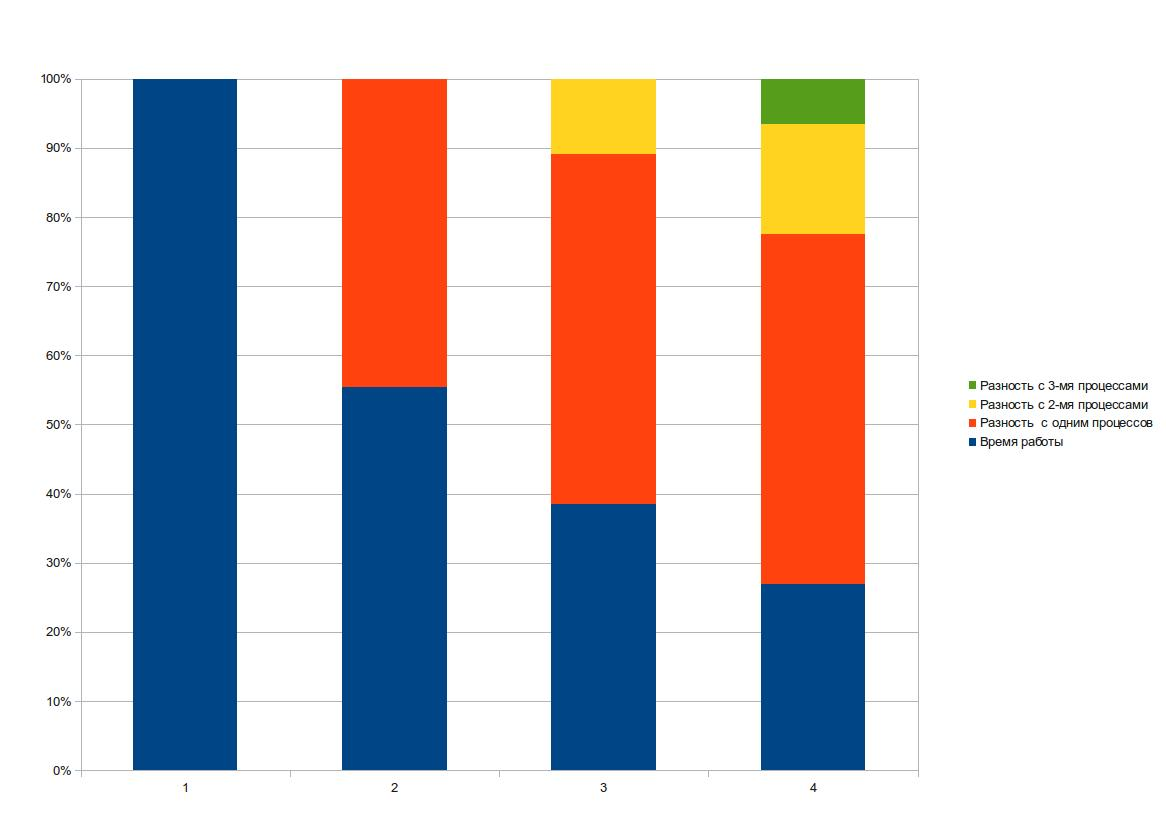
\includegraphics[width=0.7\linewidth]{images/img4.jpg}}
				\caption{ Время работы программы } 
				\label{parall_results}
	    \end{figure}
	    
\section{Результаты\label{chapter_2}}
	В качестве примера рассмотрим деформирование мембраны из алюминиевого сплава Д16T при $400^\circ\text{C}$ [\ref{teraud}]. Константы материала: 
   $C=9.37\cdot10^5 \text{МПа}^{-n}\text{сек}^{-1}$, $n=3.4$, $\sigma_b = 88.3\; \text{МПа}$. 
   Геометрические размеры мембраны: ширина $2a=200$ мм, толщина $H_0=2$ мм,$k$=1.5, $\overline{b}$=4.5 давление $q=2.65$ кПа [\ref{teraud}].  
   
   Вычисления показали, что мембрана в условиях идеального скольжения полностью заполняет криволинейную матрицу $y=4.5(1-x^{1.5})$ за бесконечное время. 
   Стадия мгновенного деформирования характеризуется параметром $\overline{H}_1 = 0.97$, 
   стадия свободного деформирования характеризуется параметрами $\overline{H}_2 = 0.69, \overline{t}_2 = 5.36 \cdot 10^8$.
   На рис.\ref{quad_sliging} представлен график зависимости толщины мембраны и интенсивности напряжения от времени
   (кривые 1 и 2 соответственно).
   
   		\begin{figure}[h!]	
				\def\svgwidth{\columnwidth}
				\center{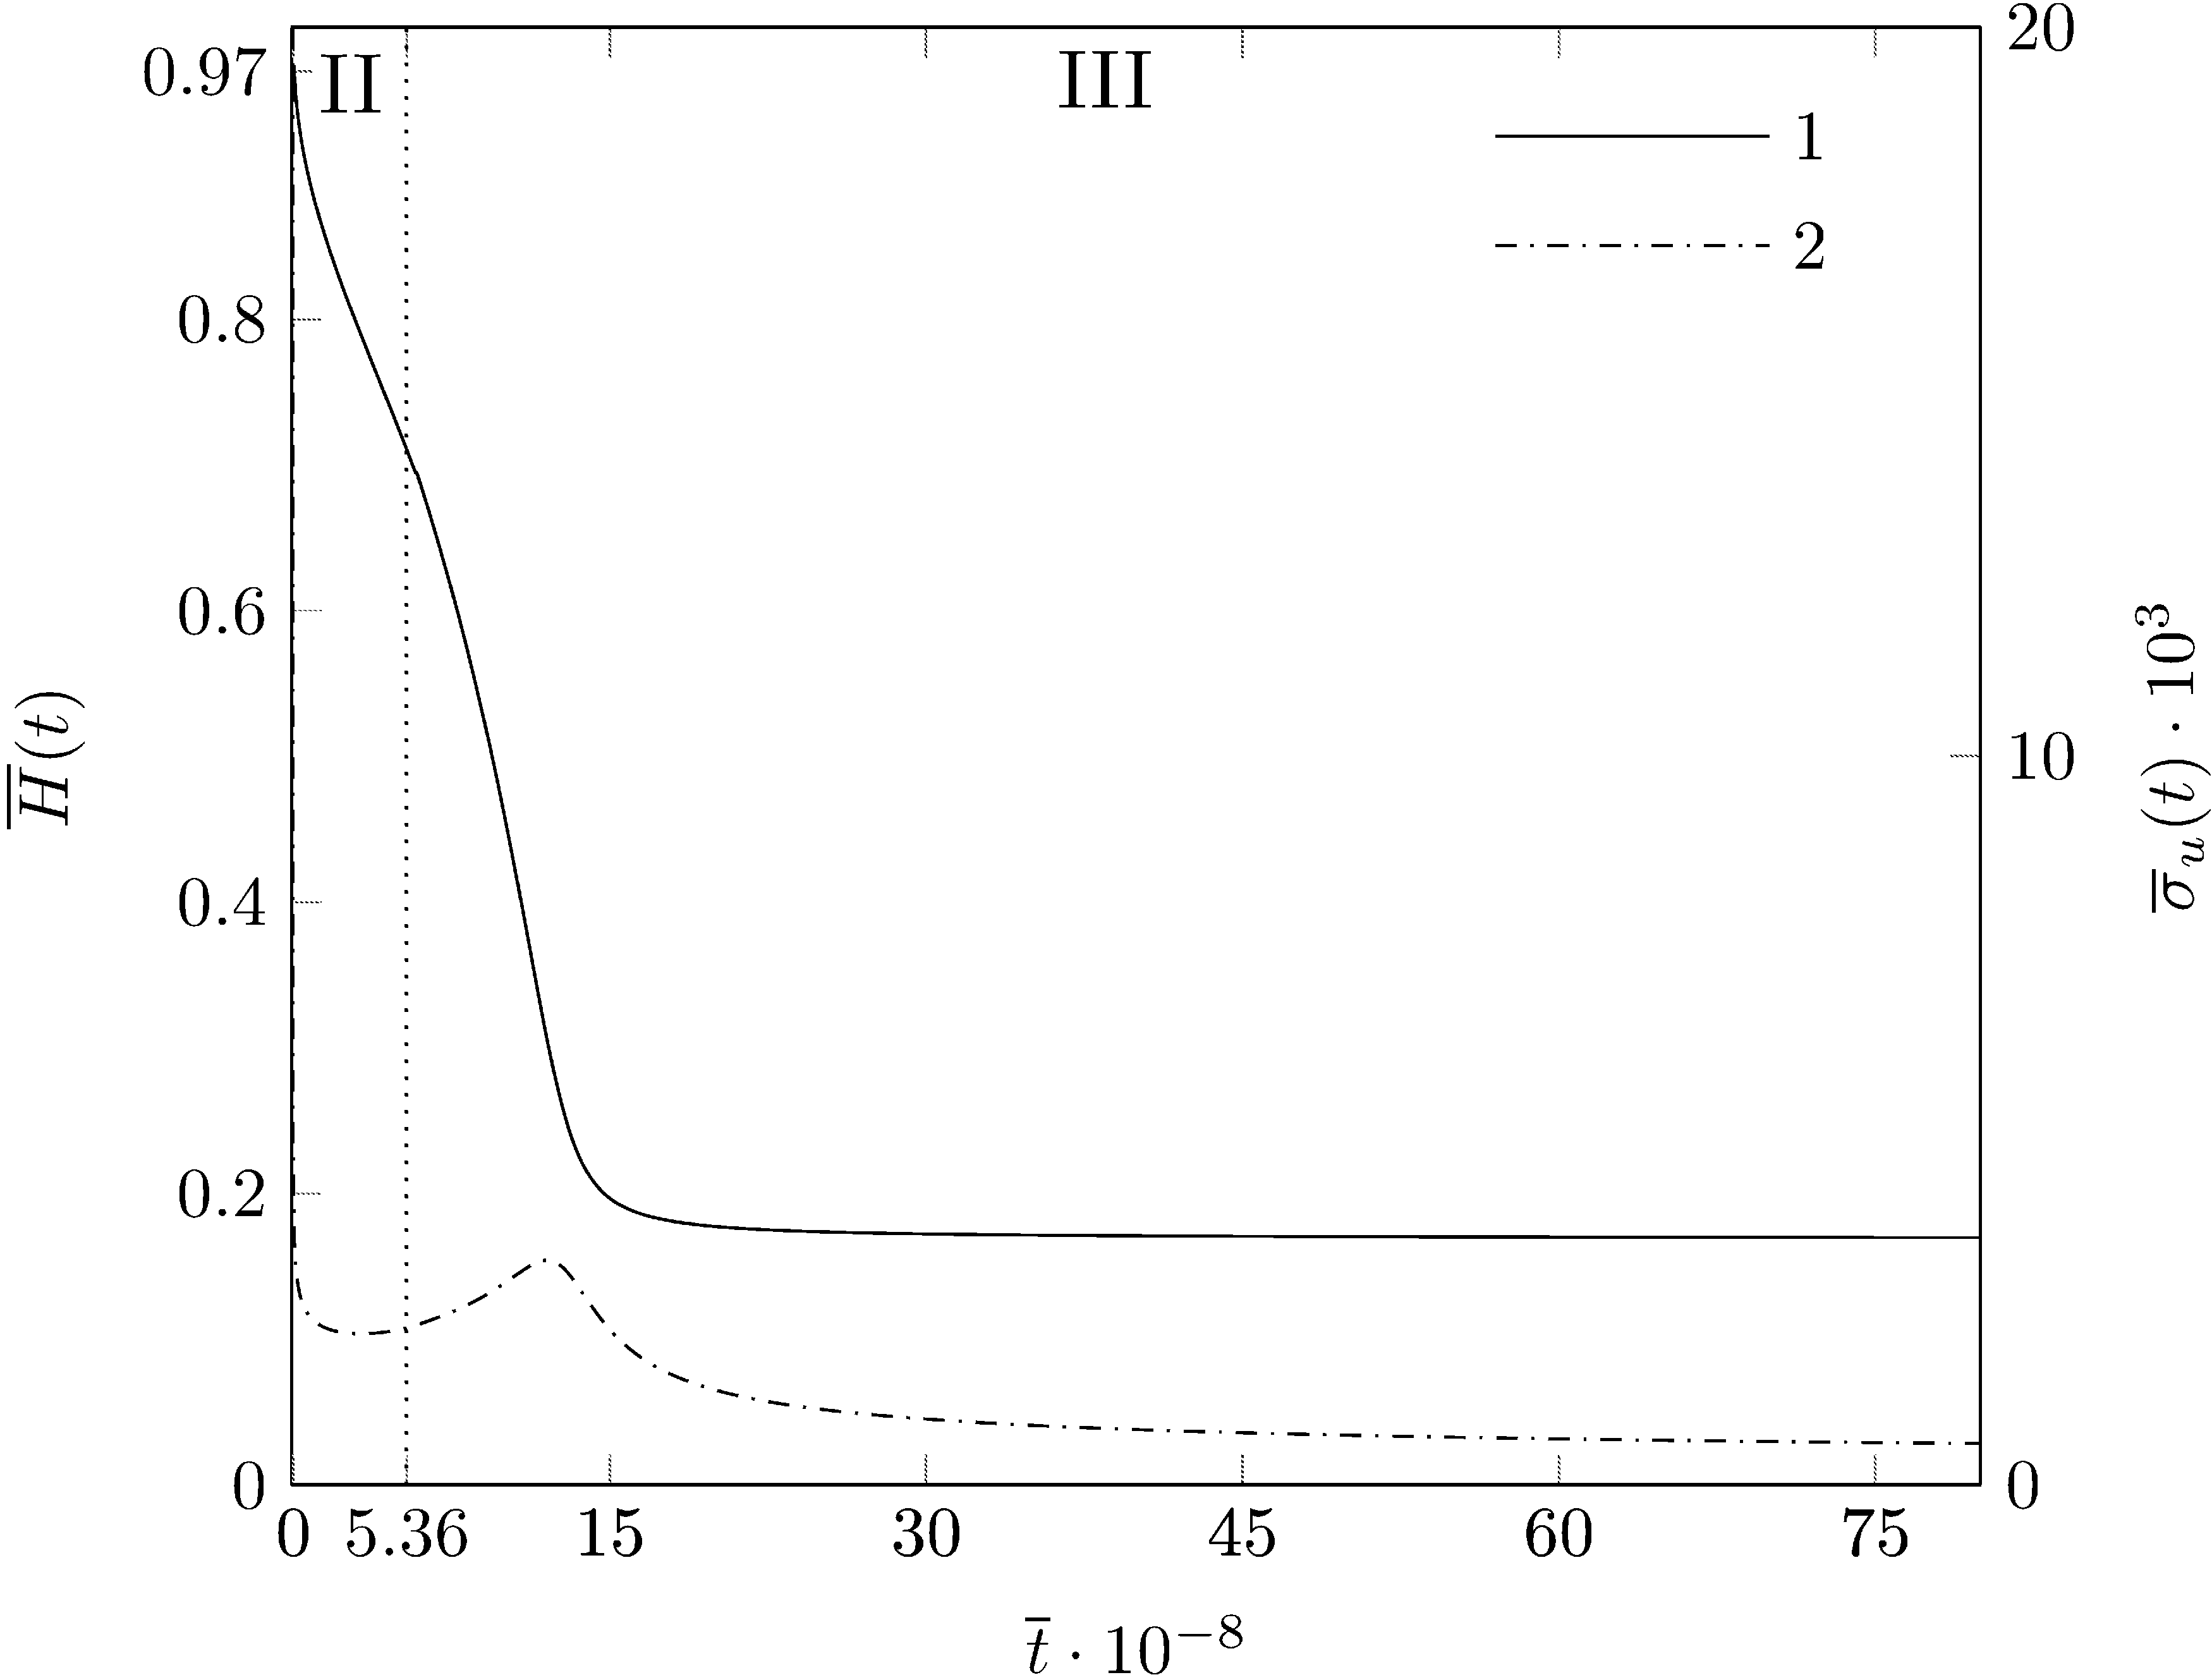
\includegraphics[width=0.7\linewidth]{images/quad_sliding.png}}
				\caption{} 
				\label{quad_sliging}
		\end{figure}
		
		Расчет для мембраны внутри матрицы с вертикальными стенками и плоским днищем проводился для матриц с различной высотой:
		$b = a$ (рис\ref{vert_sliging_ba}), $b = 4.5a$ (рис\ref{vert_sliging_4ba}),$b=7a$ (рис\ref{vert_sliging_7ba}), $b=10a$ рис\ref{vert_sliging_10ba}). При превышении высоты матрицы в 7.15 раз её ширины, при заданной толщине, происходит разрушение 
		мембраны.
		\begin{figure}[h!]	
				\def\svgwidth{\columnwidth}
				\center{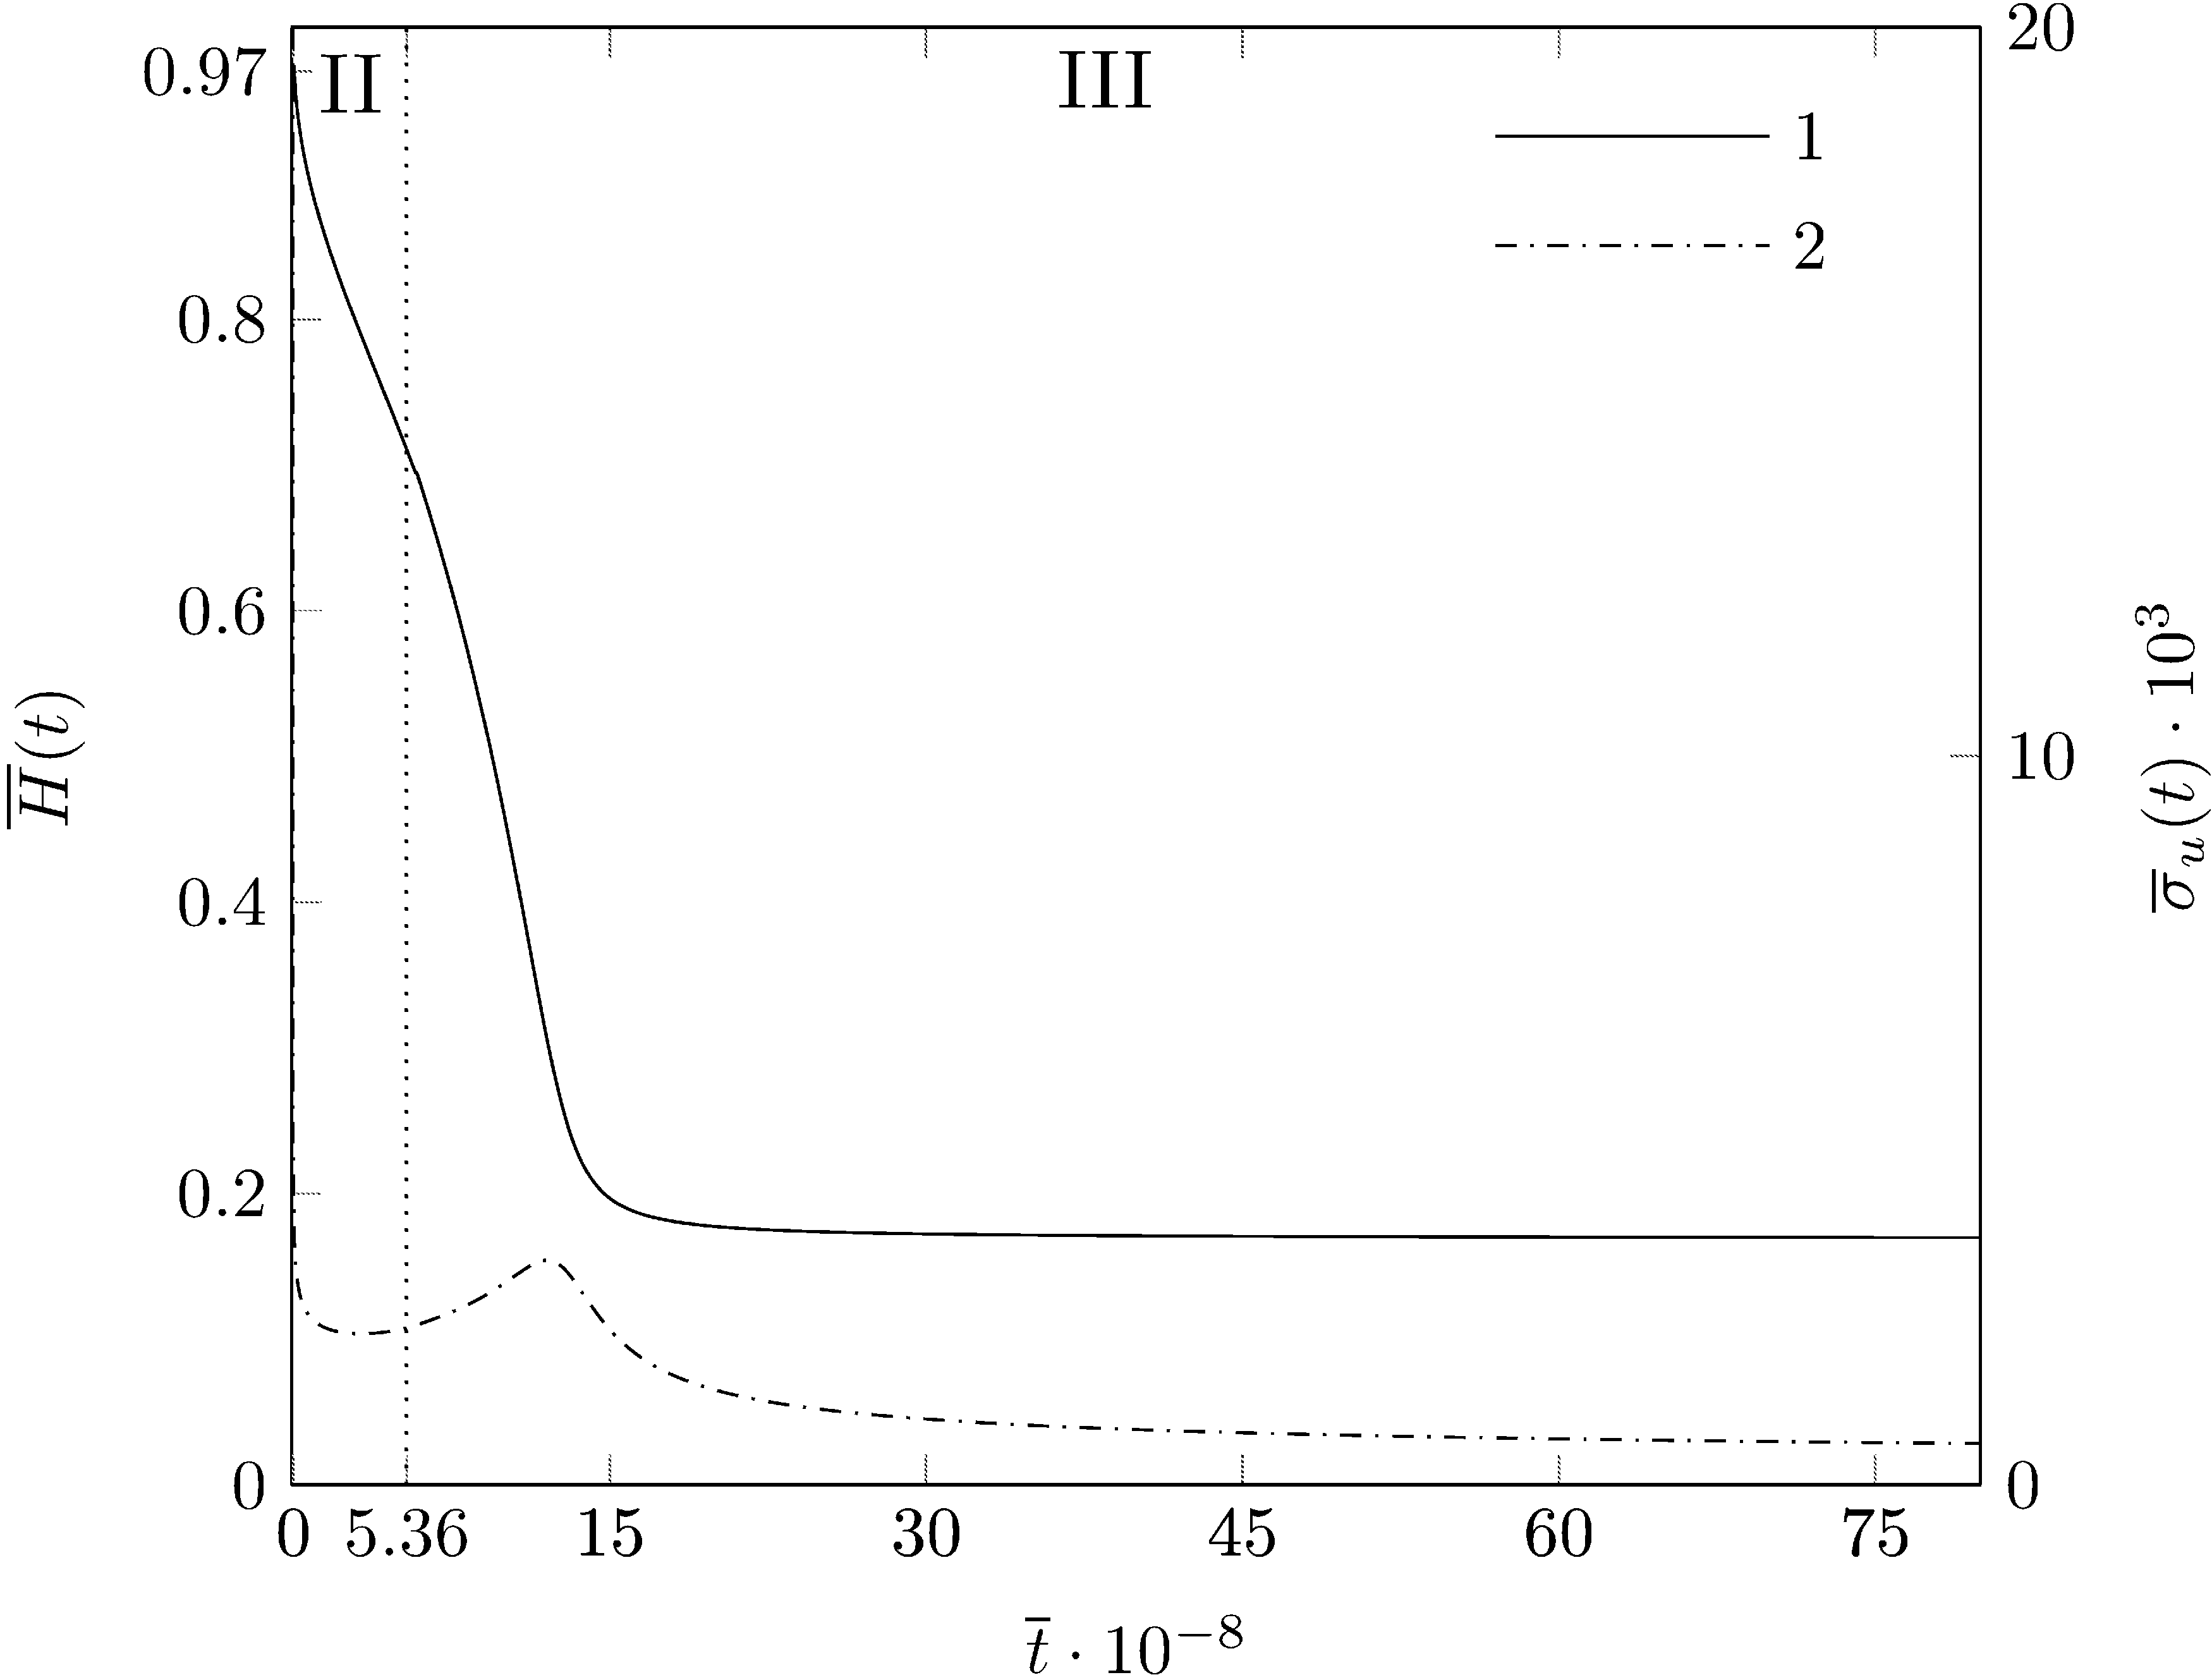
\includegraphics[width=0.7\linewidth]{images/quad_sliding.png}}
				\caption{b=a} 
				\label{vert_sliging_ba}
		\end{figure}
		\begin{figure}[h!]	
				\def\svgwidth{\columnwidth}
				\center{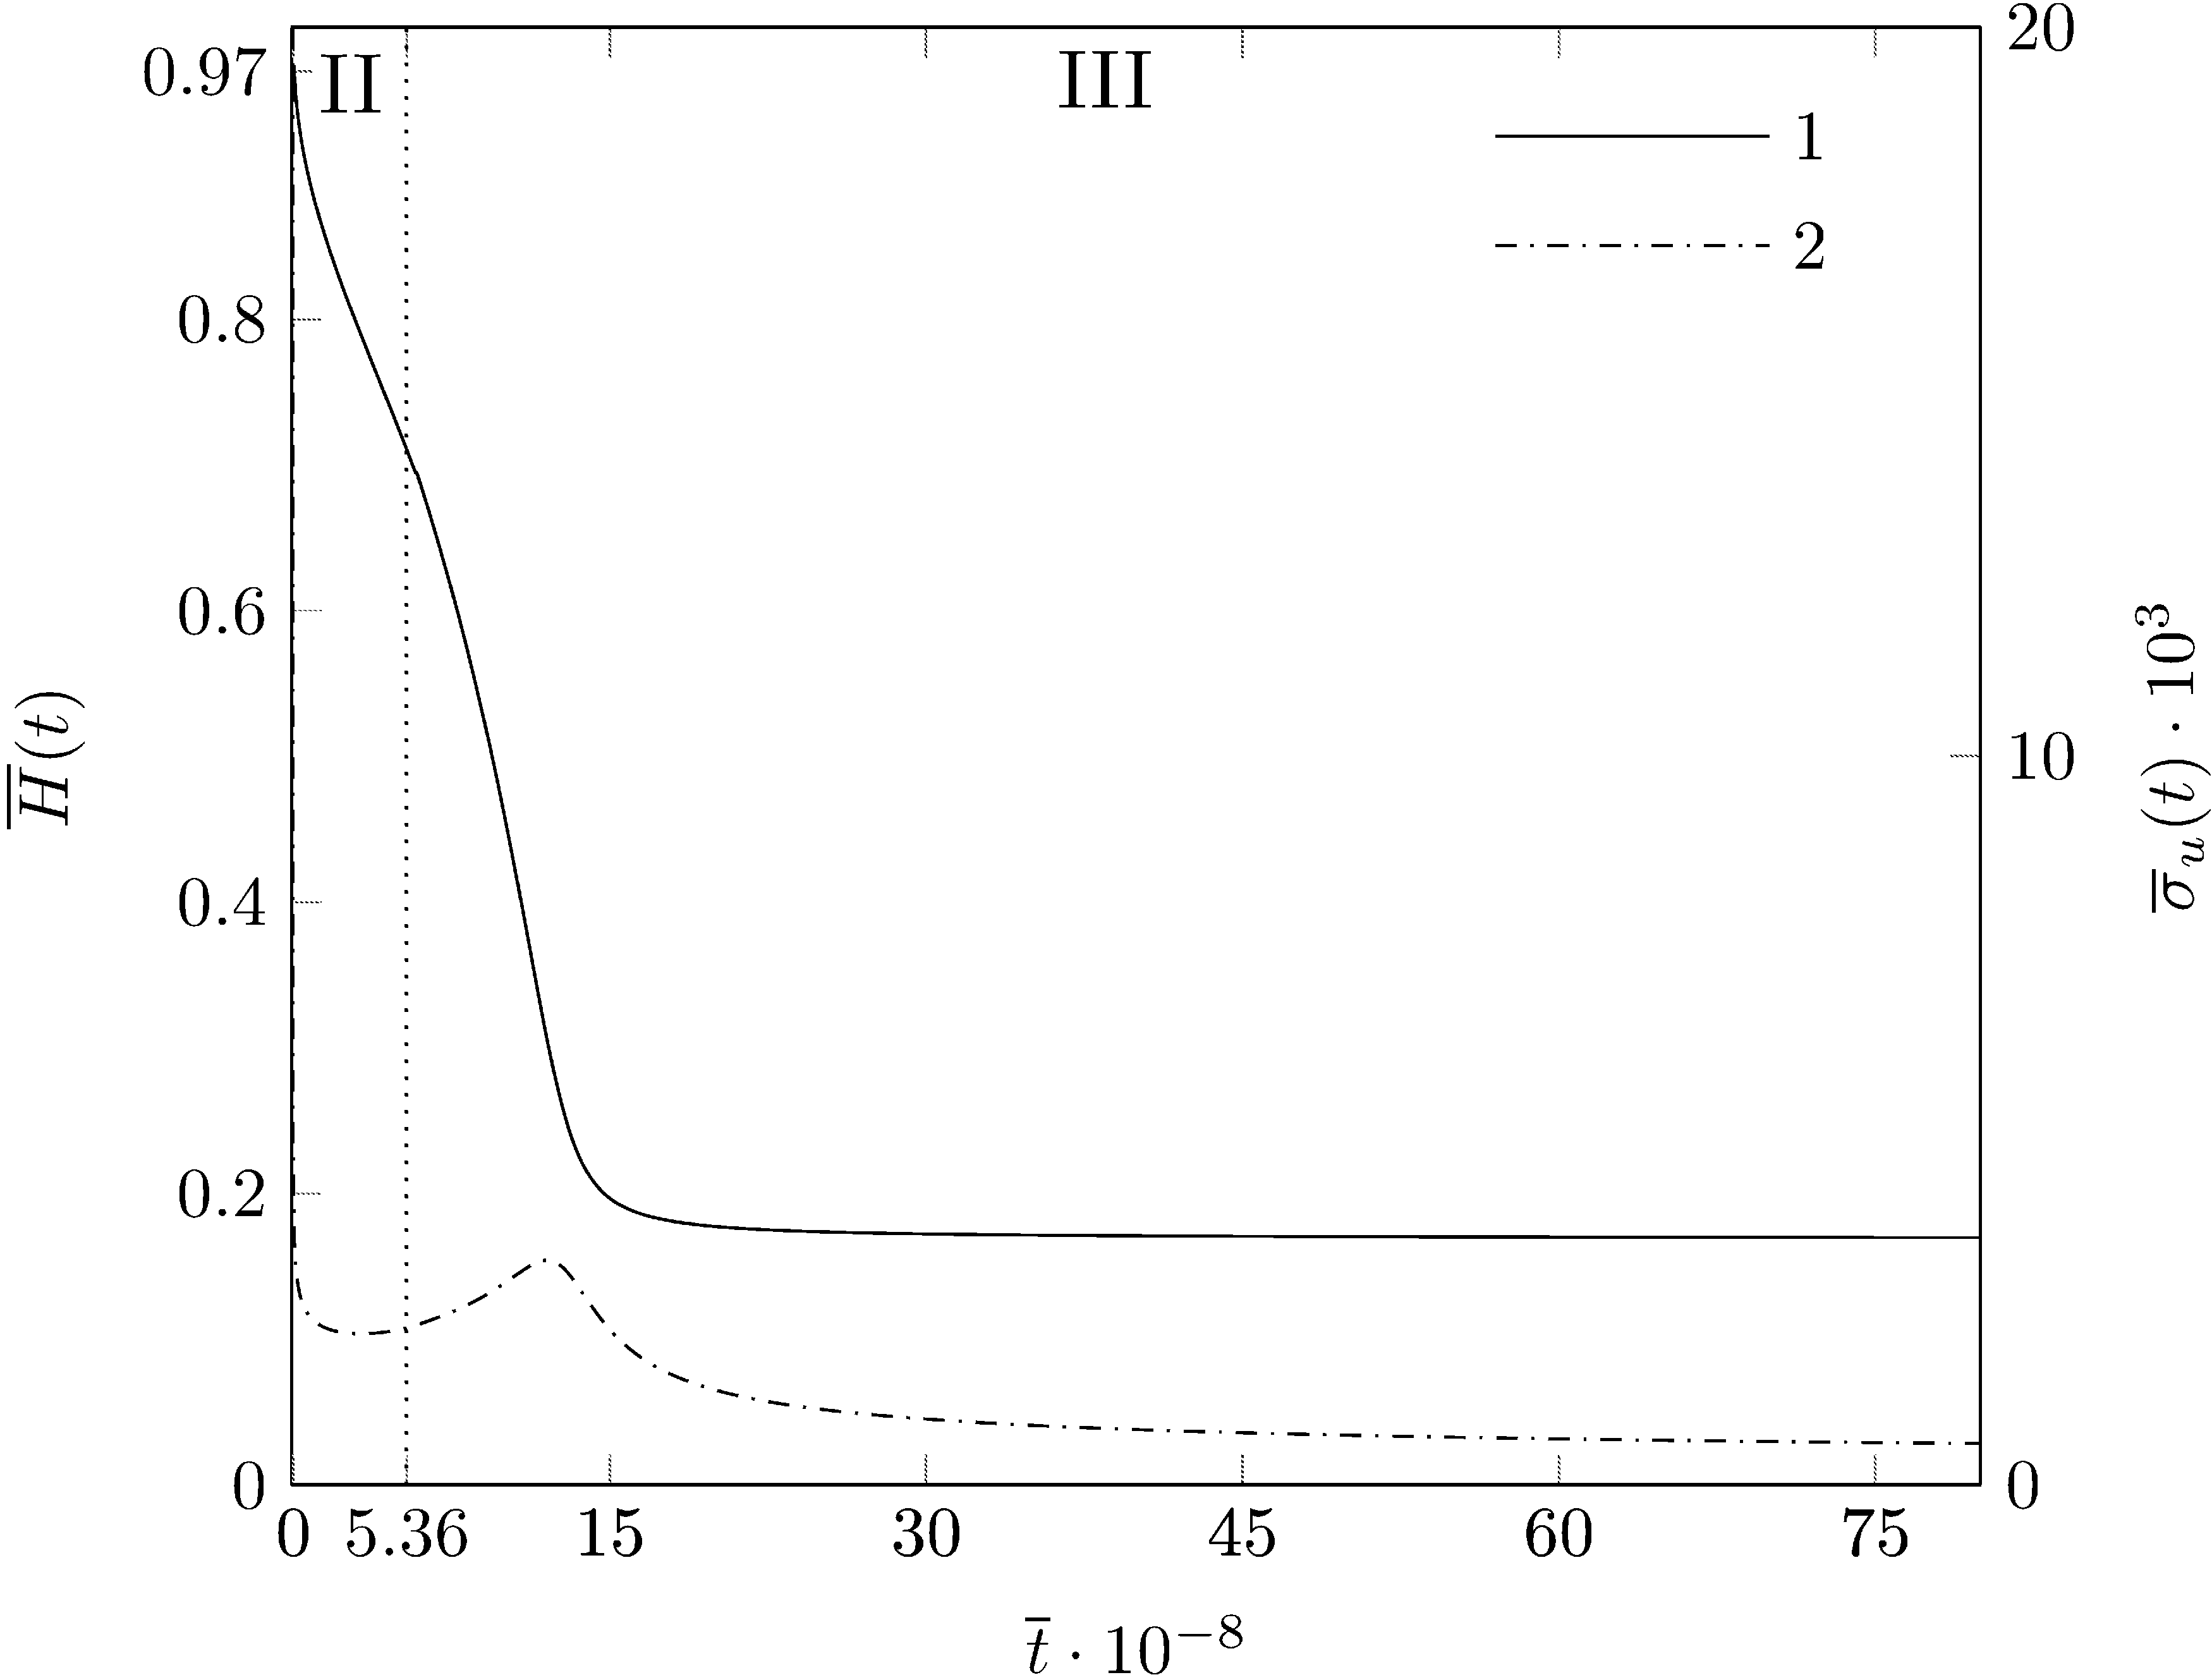
\includegraphics[width=0.7\linewidth]{images/quad_sliding.png}}
				\caption{b=a} 
				\label{vert_sliging_4ba}
		\end{figure}
				\begin{figure}[h!]	
				\def\svgwidth{\columnwidth}
				\center{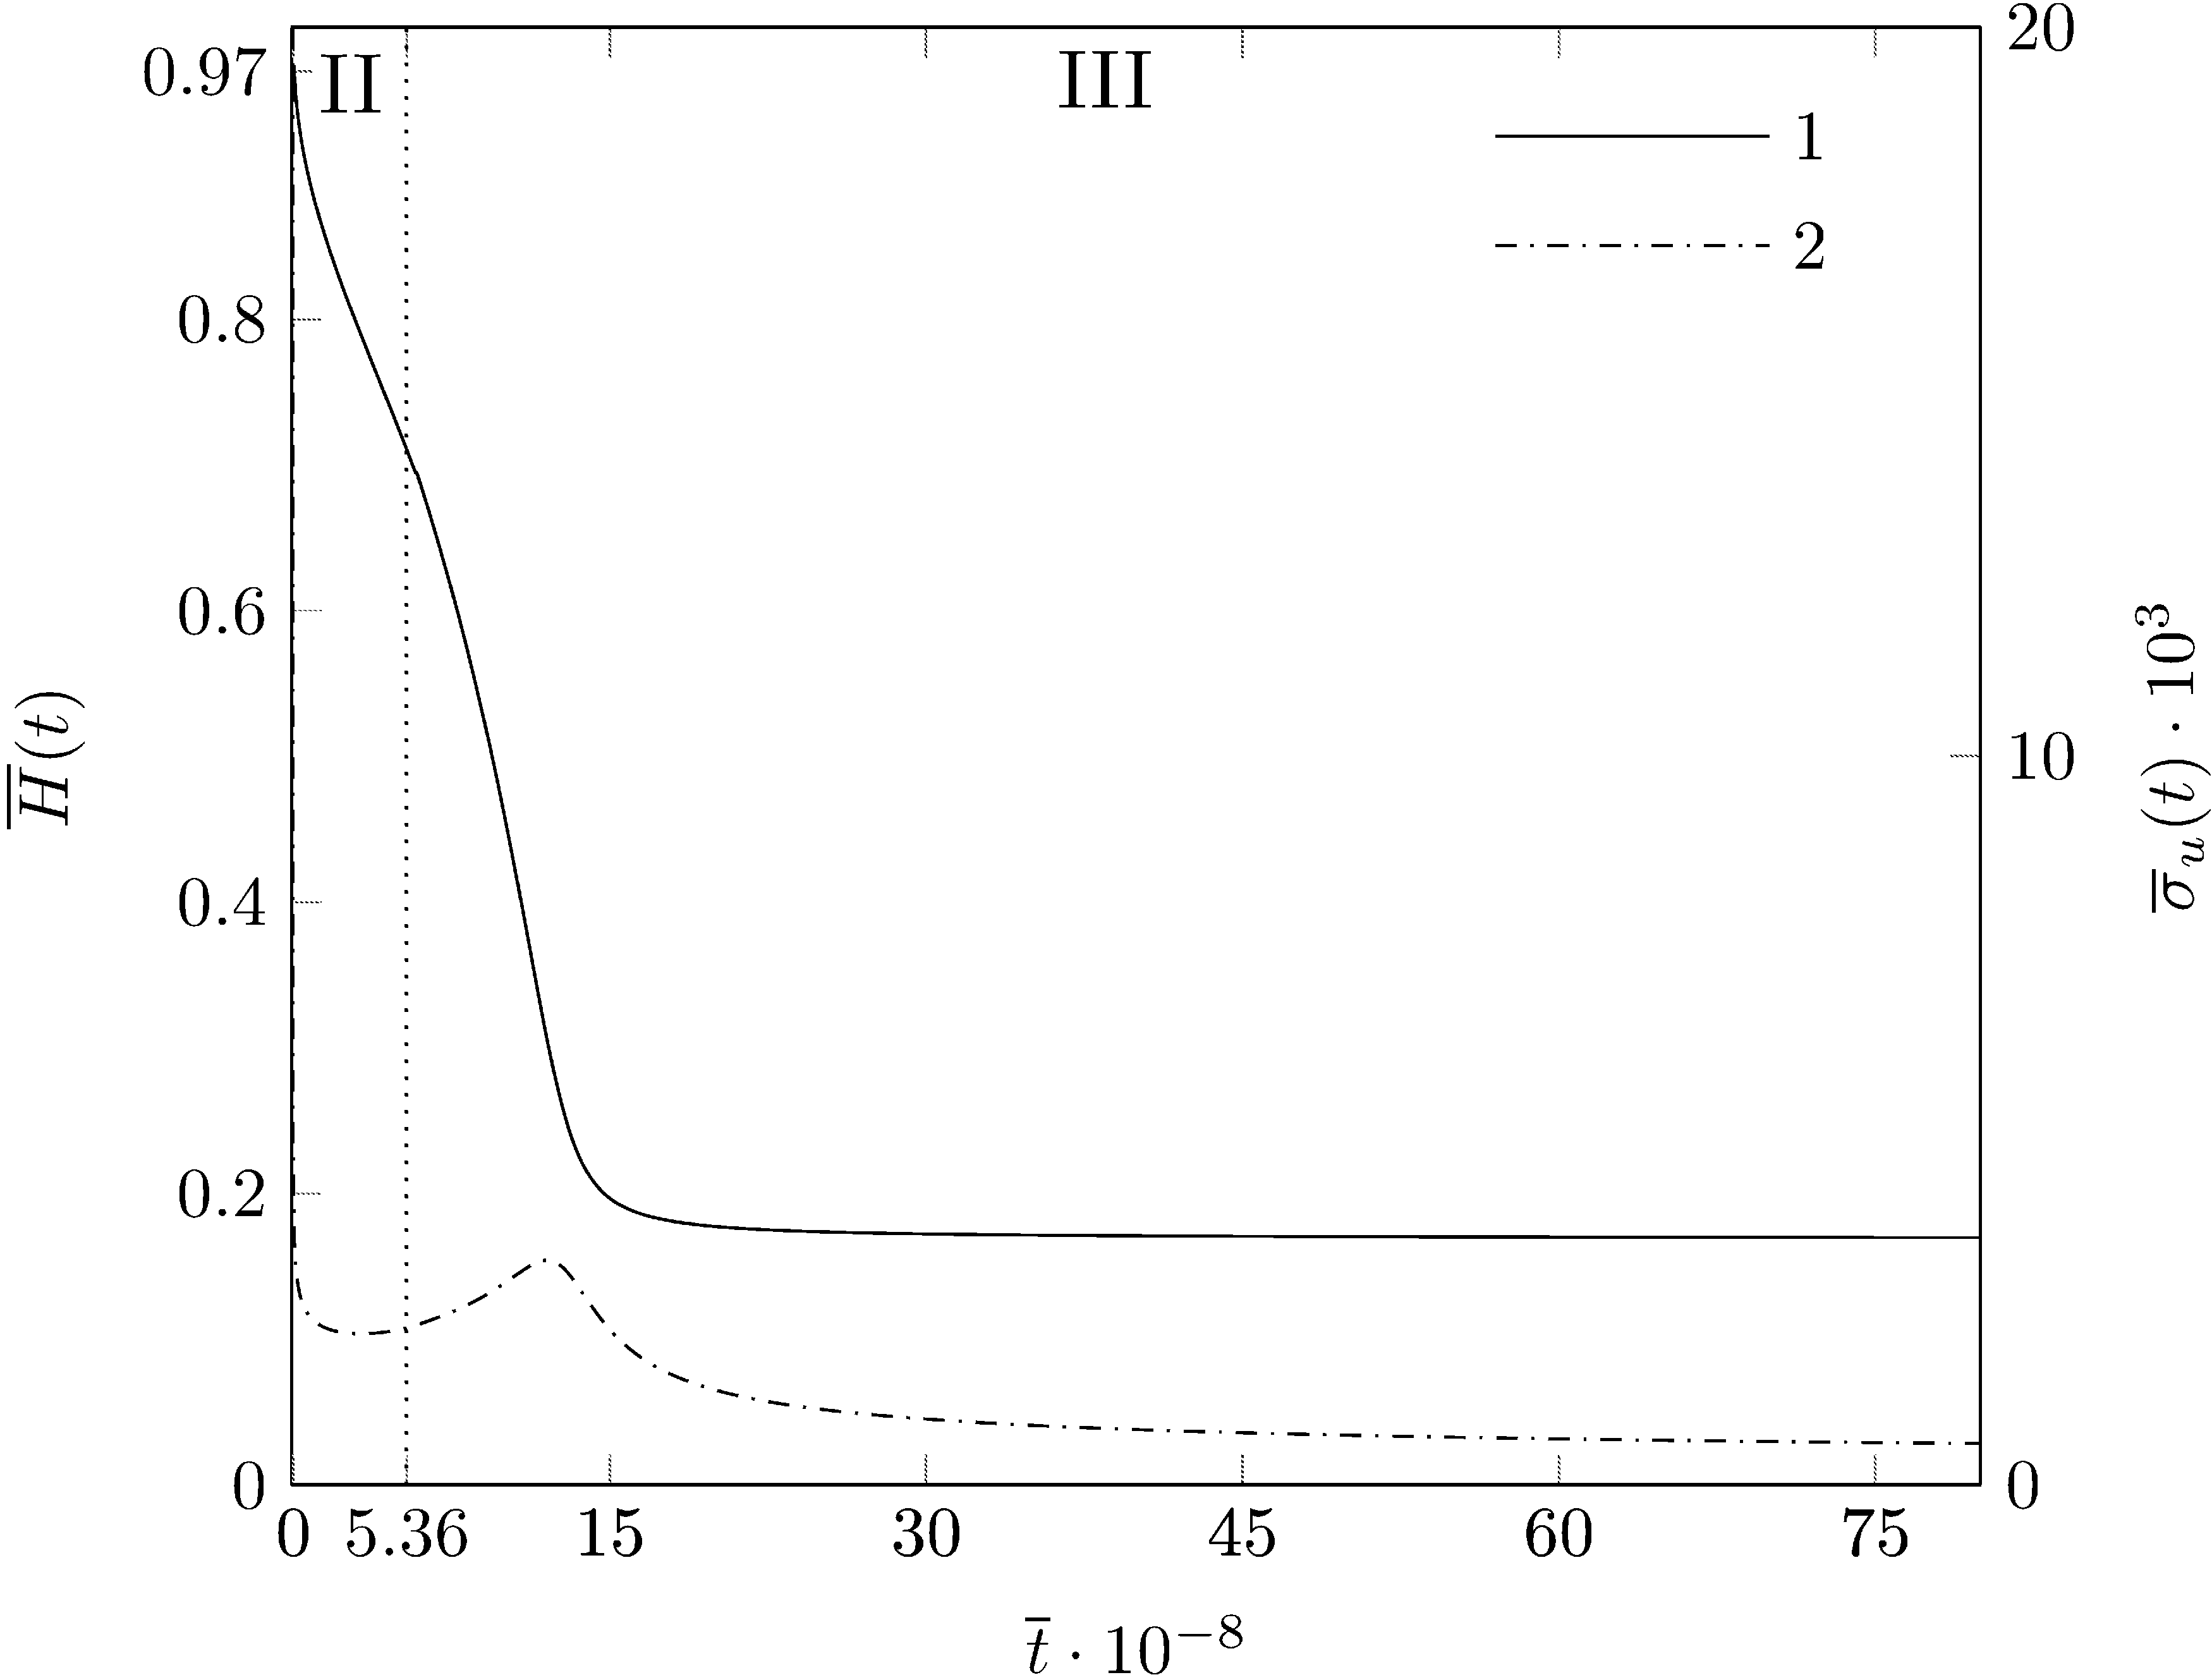
\includegraphics[width=0.7\linewidth]{images/quad_sliding.png}}
				\caption{b=a} 
				\label{vert_sliging_7ba}
		\end{figure}
				\begin{figure}[h!]	
				\def\svgwidth{\columnwidth}
				\center{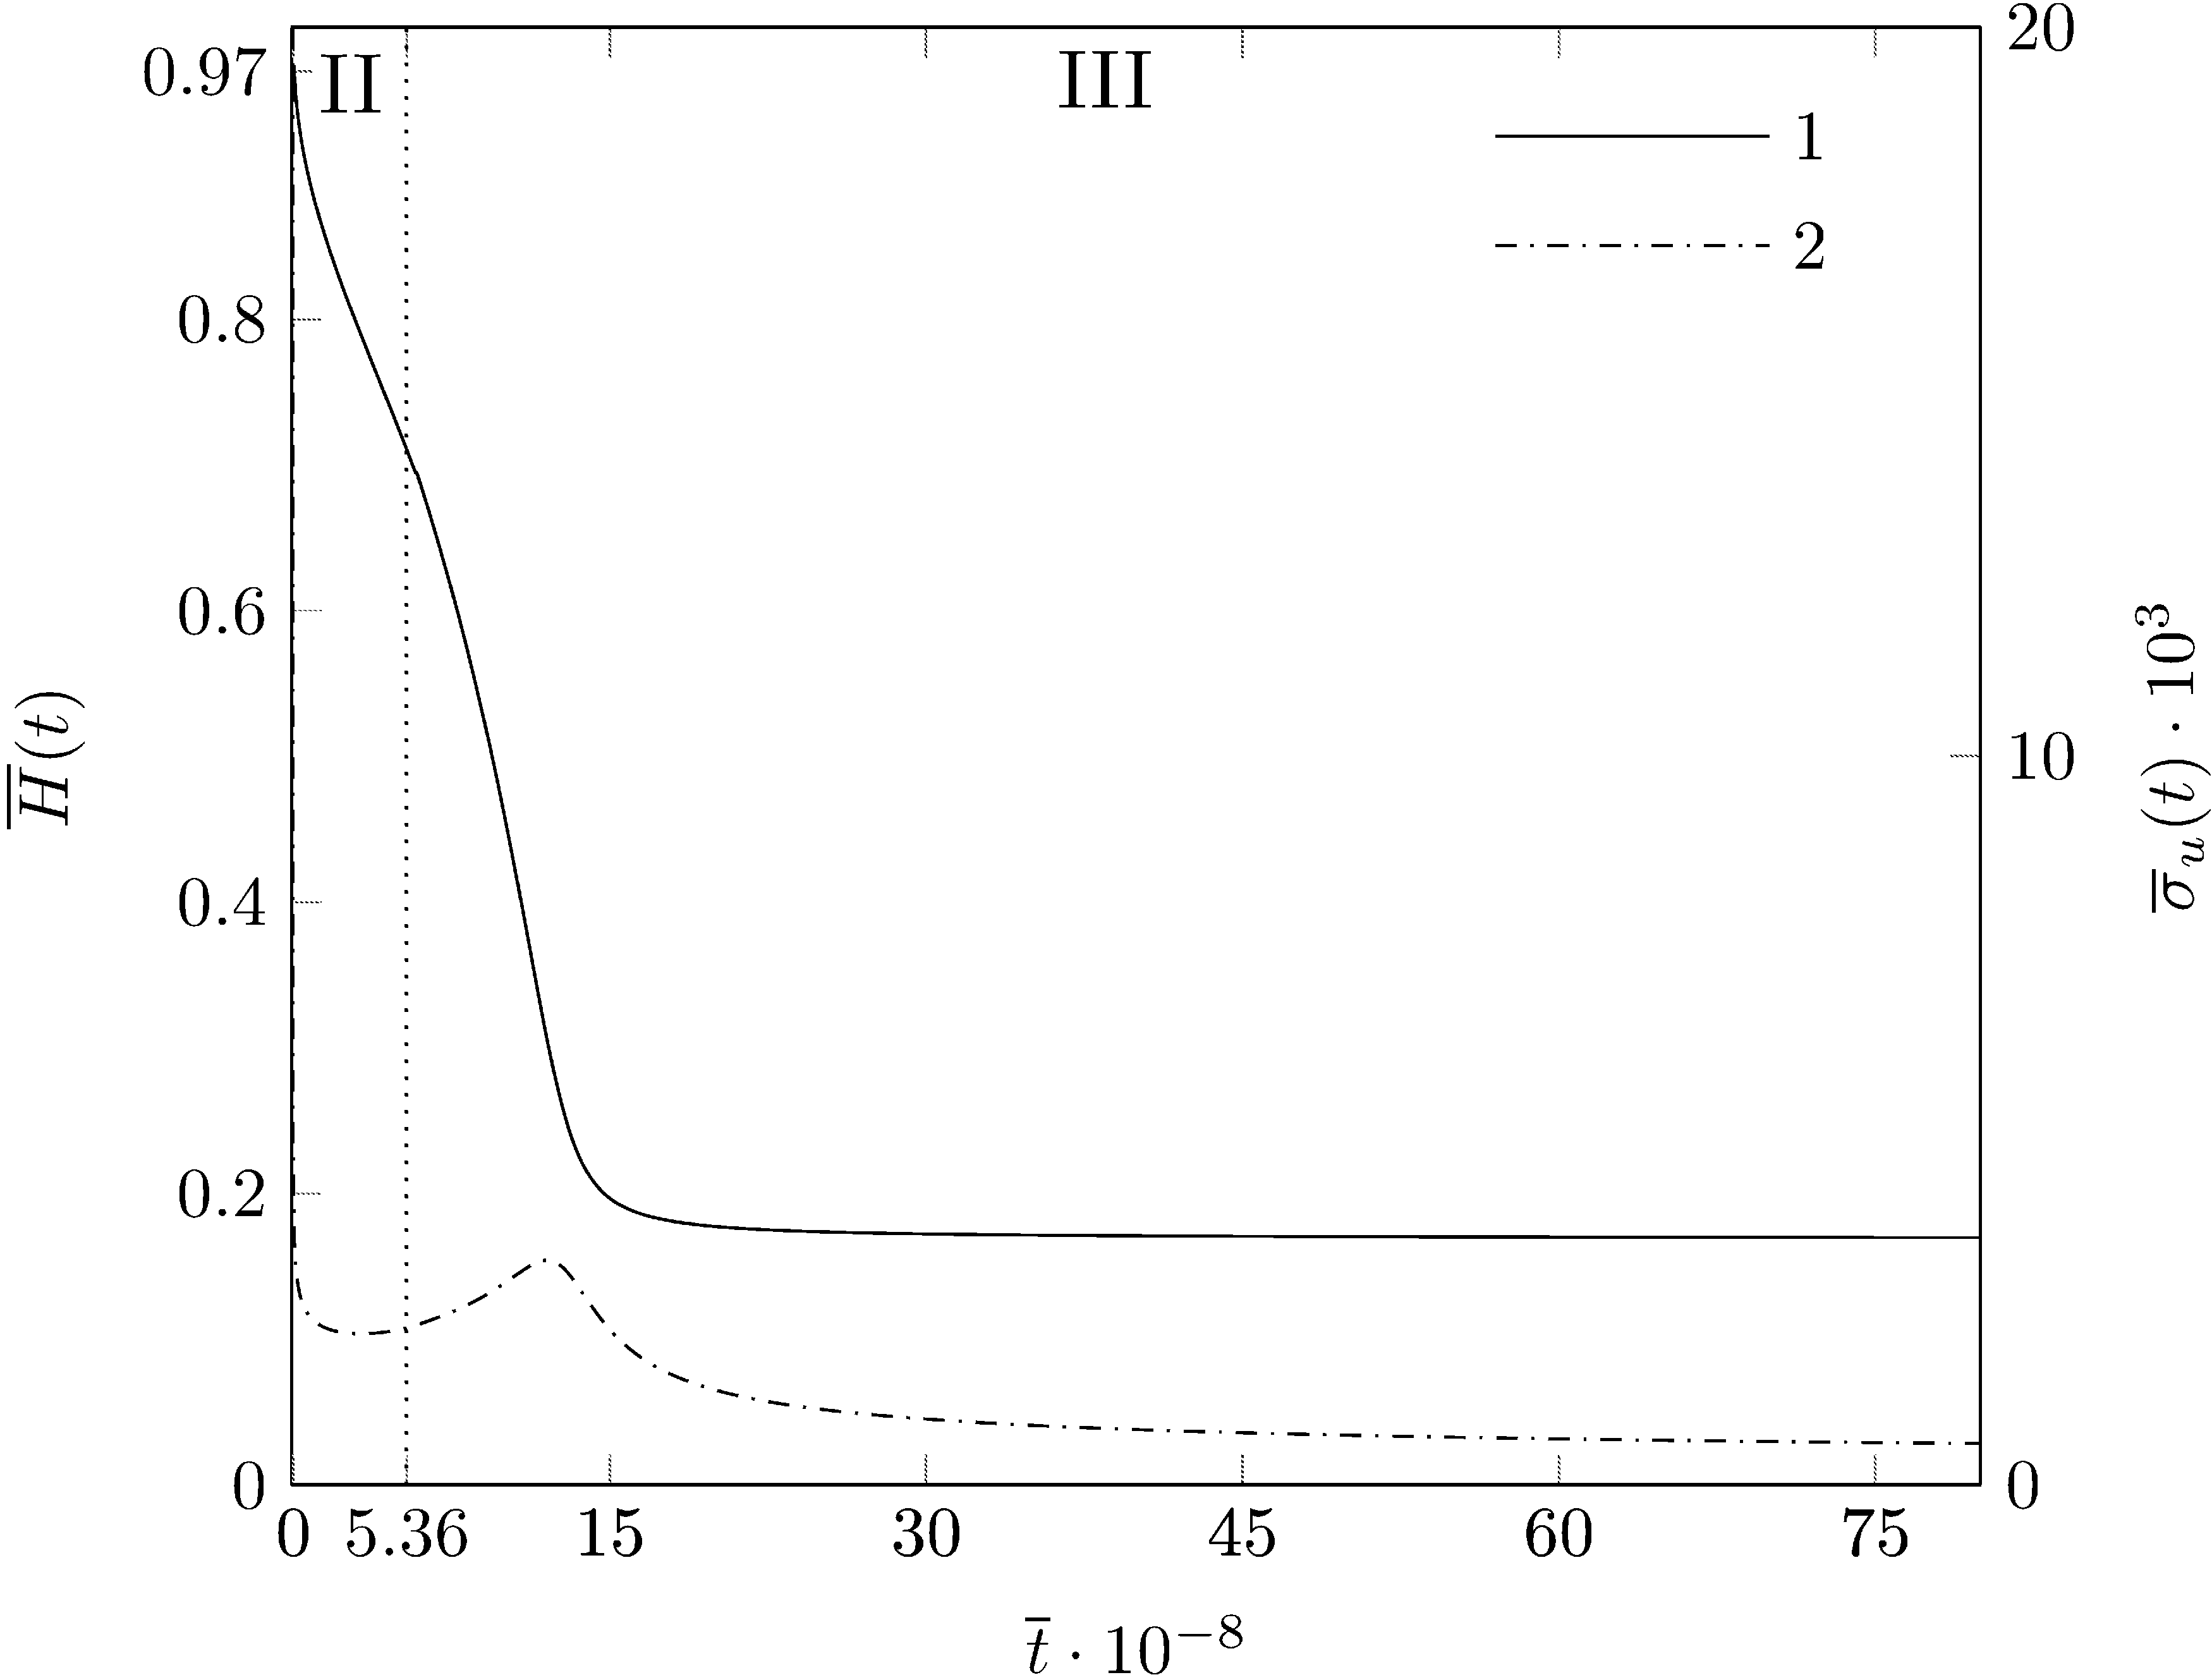
\includegraphics[width=0.7\linewidth]{images/quad_sliding.png}}
				\caption{b=a} 
				\label{vert_sliging_10ba}
		\end{figure}		
\section{Анимирование}
